\documentclass{beamer}
\usetheme{Boadilla}

\usepackage[utf8]{inputenc}
\usepackage[french]{babel} %pour la typographie française.
\usepackage[T1]{fontenc} %pour la césure des mots.
\usepackage{amssymb} %pour les symboles mathématiques et lettres grecques
\usepackage{amsmath} %pour les formules mathématiques avancées

\beamertemplatenavigationsymbolsempty % Flag nazi pour supprimer la ligne d'option dans les slides

\title{Projet TriComp : Présentation}
\author{Equipe TriComp}
\date{Jeudi 18 Décembre 2014}

\begin{document}

\frame{
   \begin{center}
        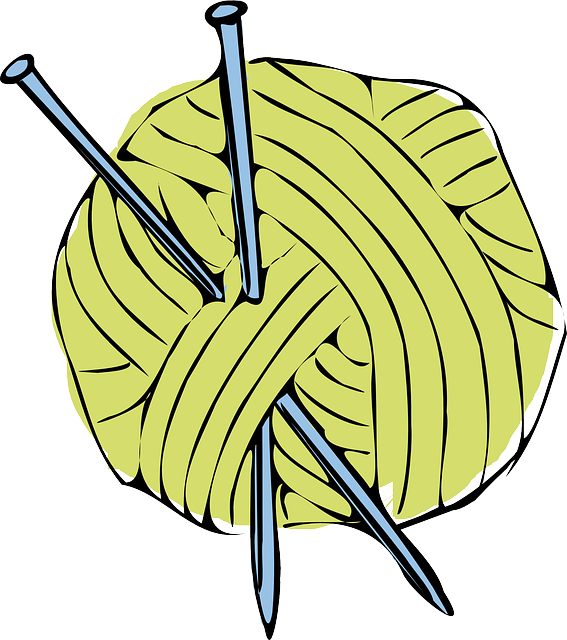
\includegraphics[height=0.2\textheight]{../img/ball_of_wool.png}
        \hspace*{4cm}
        
\includegraphics[height=0.2\textheight]{../img/ens.jpg}
   \end{center}
   \titlepage
}

\frame{
	\frametitle{Plan} 
		\tableofcontents
}

\section{Introduction}

\subsection{L'équipe}

\frame{
	\frametitle{L'équipe TriComp}
		\begin{center}
			{\large
			{William \textsc{Aufort} \hspace{4cm} Julien \textsc{Bensmail} \\}
			\vspace{1cm}
			{Agathe \textsc{Herrou}  \hspace{4cm} Romain \textsc{Labolle} \\}
			\vspace{1cm}
			{Frédéric \textsc{Lang} \hspace{4cm} Maxime \textsc{Lesourd} \\}
			\vspace{1cm}       
			{Laureline \textsc{Pinault} \hspace{3.7cm} Léo \textsc{Stéfanesco} \\}}
		\end{center}
}

\subsection{Présentation générale}

\frame{
	\frametitle{Présentation générale}
		% TriComp = Tricot + Compilateur
		% Tricot -> logiciel pour tricoteur
		% Compilateur -> réalisation du tricot
		% ==> Un logiciel d'édition de tricot, mais surtout de génération d'instructions 
}

\subsection{Motivations}

\frame{
	\frametitle{Motivations}
		% Logiciels de tricot actuels : beaucoup d'édition, mais 
		% Livre de tricot : difficiles à suivre ? Pas spécifique à une pièce en particulier.
		% Originalité.		
		% Autres ...
}

\frame{
	\frametitle{Quelques notions de tricot...}
}

% Proposition de plan :
% Introduction : présentation de l'équipe, 
% TriComp : Origine de l'idée, Compilateur ? Tricot ?
% Travail en amont : Problèmes à résoudre (allocation aiguilles, qqchose de général) -> "langage haut niveau"
% Coté logiciel : interface
% Difficultés rencontrées
% Améliorations possibles (complexifier fonctionnalites, reprendre les objectifs non traités du midterm)

\section{Notre travail}

\subsection{Conception d'un langage descriptif}

\frame{
	\frametitle{En amont... description d'un tricot}
		\begin{itemize}
			\item Un schéma de description de nimporte quel tricot
			\item Plusieurs critères :
			\begin{itemize}
				\item facilité pour générer les instructions
				\item assez "haut niveau" % i.e : suffisamment précis pour avoir du détail, mais conserver un aspect global, contrairement
										  % à ce qui se fait d'habitude dans les logiciels de tricots (points sur une grille)
				\item facile de compréhension et d'utilisation (notamment dans le code...)
			\end{itemize}
			\item Nous avons donc conçu le langage TriLang % TODO : meilleur nom ?
		\end{itemize}
}

\frame{
	\frametitle{Le langage}
		\begin{itemize}
			\item La composante essentielle : le trapèze
			\item Pour relier/séparer des pièces : \texttt{link} et \texttt{split}
			\item Un exemple
			% TODO : Exemple
		\end{itemize}
}	

\subsection{Conception d'un compilateur}

\frame{
	\frametitle{Le compilateur}
		\begin{itemize}
			\item Pouvoir passer d'un tricot à la liste des instructions pour le réaliser
			\item Mais aussi des étapes intermédiaires :
			\begin{itemize}
				\item Vérifications 
			    \item Allocation d'aiguilles ? % TODO est ce que ca sera fait ?
			\end{itemize}
		\end{itemize}
}

\subsection{Elaboration d'une interface}

\frame{
	\frametitle{L'interface graphique}
		\begin{itemize}
			\item Simple d'utilisation
			\item Outils d'éditions
			\item Appel au compilateur
		\end{itemize}
}

\frame{
	\begin{center}
		\Huge{Démo !}
	\end{center}
}

\end{document}

